

%% Lee
%% In dissertation, change section* to chapter and subsection* to section


\chapter{System Description}
\label{chap-four}

% ----------------------------------------------------------------------------------------------------
% ----------------------------------------------------------------------------------------------------
%\section{ANN System}
%\label{sec:ANN System}

The primary design considerations that drove the architecture of this work are :
\begin{outline}
  \1 Target applications are unable to take advantage of memory reuse opportunities and therefore not able to achieve high performance using local \ac{sram} to store \ac{ann} parameters or the \ac{ann} input 
  \1 \ac{dram} is required for storage of \ac{ann} parameters 
  \1 Target application will likely apply many disparate \acp{ann} to perform various system functions
  \1 Target application will have space and power limitations
\end{outline}

\section{Overview}
\label{sec:chap1_overview}
This work employs \ac{3dic} technology along with a custom 3D-DRAM. The objective was to demonstrate that a pure \ac{3dic} system can implement multiple disparate \acp{ann}. By staying within the \ac{3dic} footprint and taking advantage of high
density \acp{tsv} this work is able to maintain a significantly higher bandwidth over 2D or 2.5D \ac{asic} or \ac{asip} solutions.

The \ac{3dic} system die stack (figure \ref{fig:3DICStack}) includes the 3D-\ac{dram} with a system manager below and one or more processing layers below the manager.
\begin{figure}[!t]
% the [] contains position info e.g. [!t] means here
\centering
\captionsetup{justification=centering}
\captionsetup{width=.9\linewidth}
\centerline{
\mbox{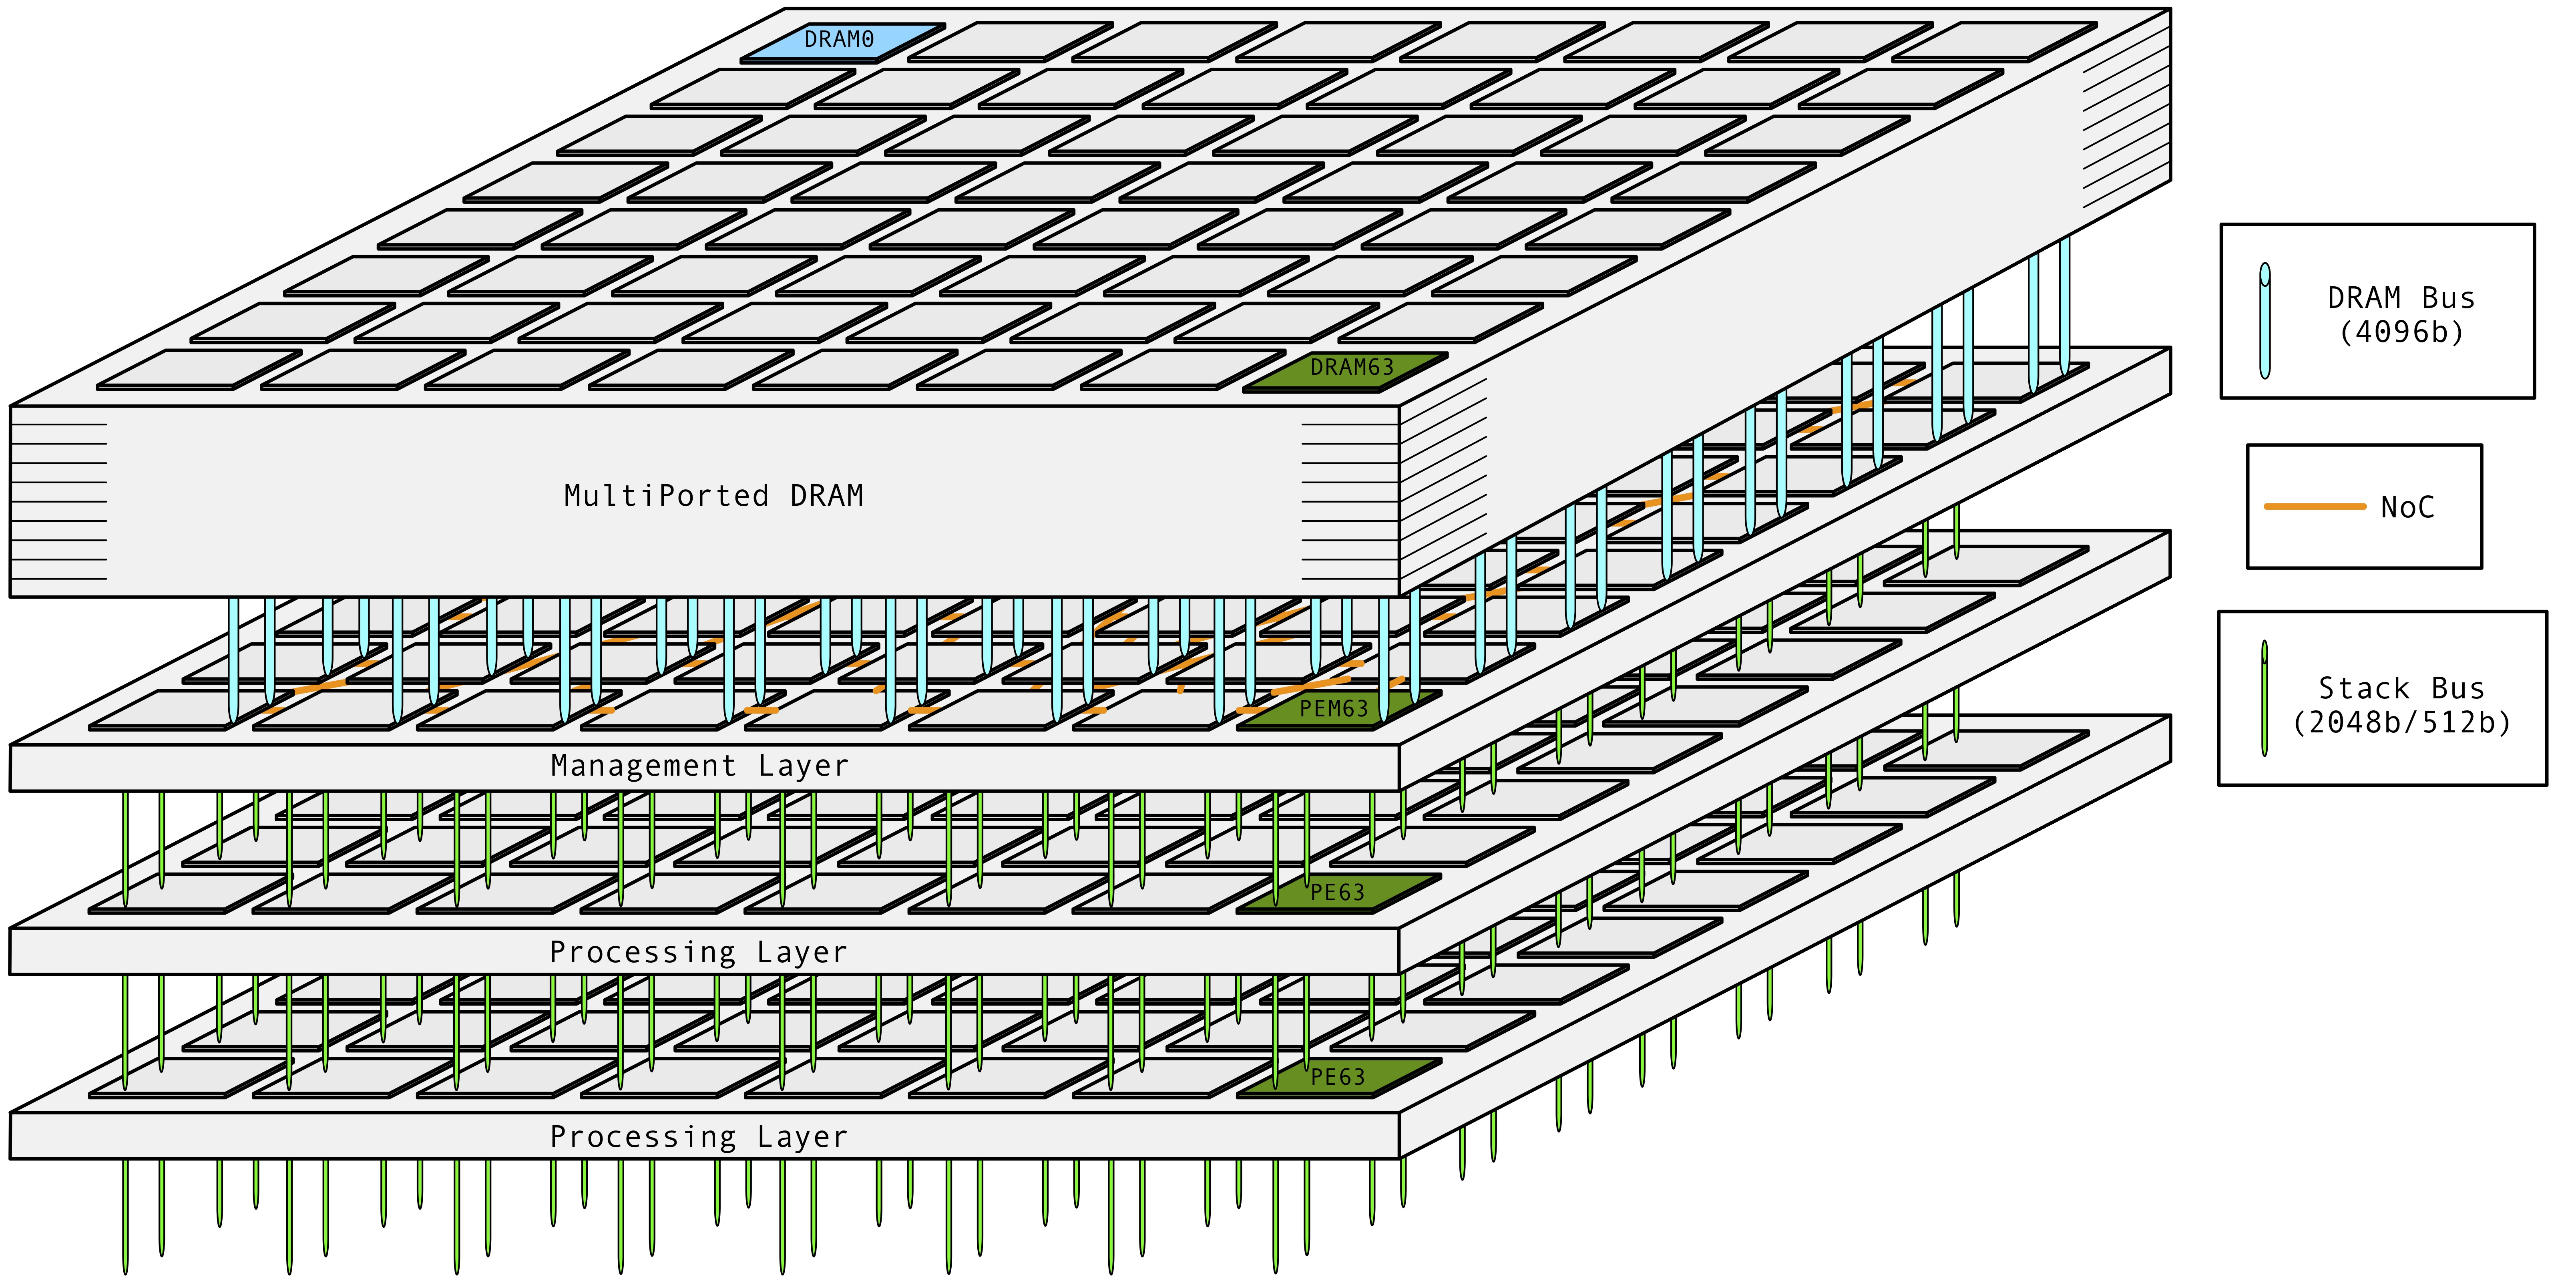
\includegraphics[width=.9\linewidth]{StackDiagram.jpg}}
}
\caption{3DIC System Stack}
\label{fig:3DICStack}
\end{figure}

3D-DRAM has recently become available in standards such as \ac{hbm} and \ac{hmc} and proprietary devices such as the DiRAM4 available from Tezzaron. 
These technologies provide high capacity within a small footprint.

In the case of \ac{hbm} and DiRAM4, the technology can be combined with additional custom layers to provide a system solution.

The question becomes, can a useful system coexist within the same 3D footprint?

This work targeted a baselne system with:
\begin{itemize}
  \item Computations require single precision floating point precision
  \item Utilize the Tezzaron DiRAM4 \ac{dram} for for main memory
\end{itemize}
The work includes customizing the interface to a 3D-\ac{dram}, researching data structures to describe storage of \ac{ann} parameters, designing a memory manager with unique micro-coded instructions and a \ac{pe} layer.  
The system is designed such that a sub-system, known as a \ac{ssc} operates on one of these disjoint memories within the 3D-\ac{dram} (see figure \ref{fig:diram4Layout}).

When the \acp{ssc} need to share data or neuron activations, the data is passed between \acp{ssc} using a \ac{noc}.

An overview of the various blocks and interconnects are given below:

% ----------------------------------------------------------------------------------------------------
\section{3D-DRAM}
The targetted 3D-\ac{dram}, the Tezzaron DiRAM4 is a 3D-\ac{dram} employs multiple memory array layers in conjunction with a control and IO layer.
The memory is formed from 64 disjoint sub-memories each providing upwards of 1Gigabit with a total capacity of at least 64 gigabit.
\begin{figure}[!t]
% the [] contains position info e.g. [!t] means here
\centering
\captionsetup{justification=centering}
\captionsetup{width=.9\linewidth}
\centerline{
\mbox{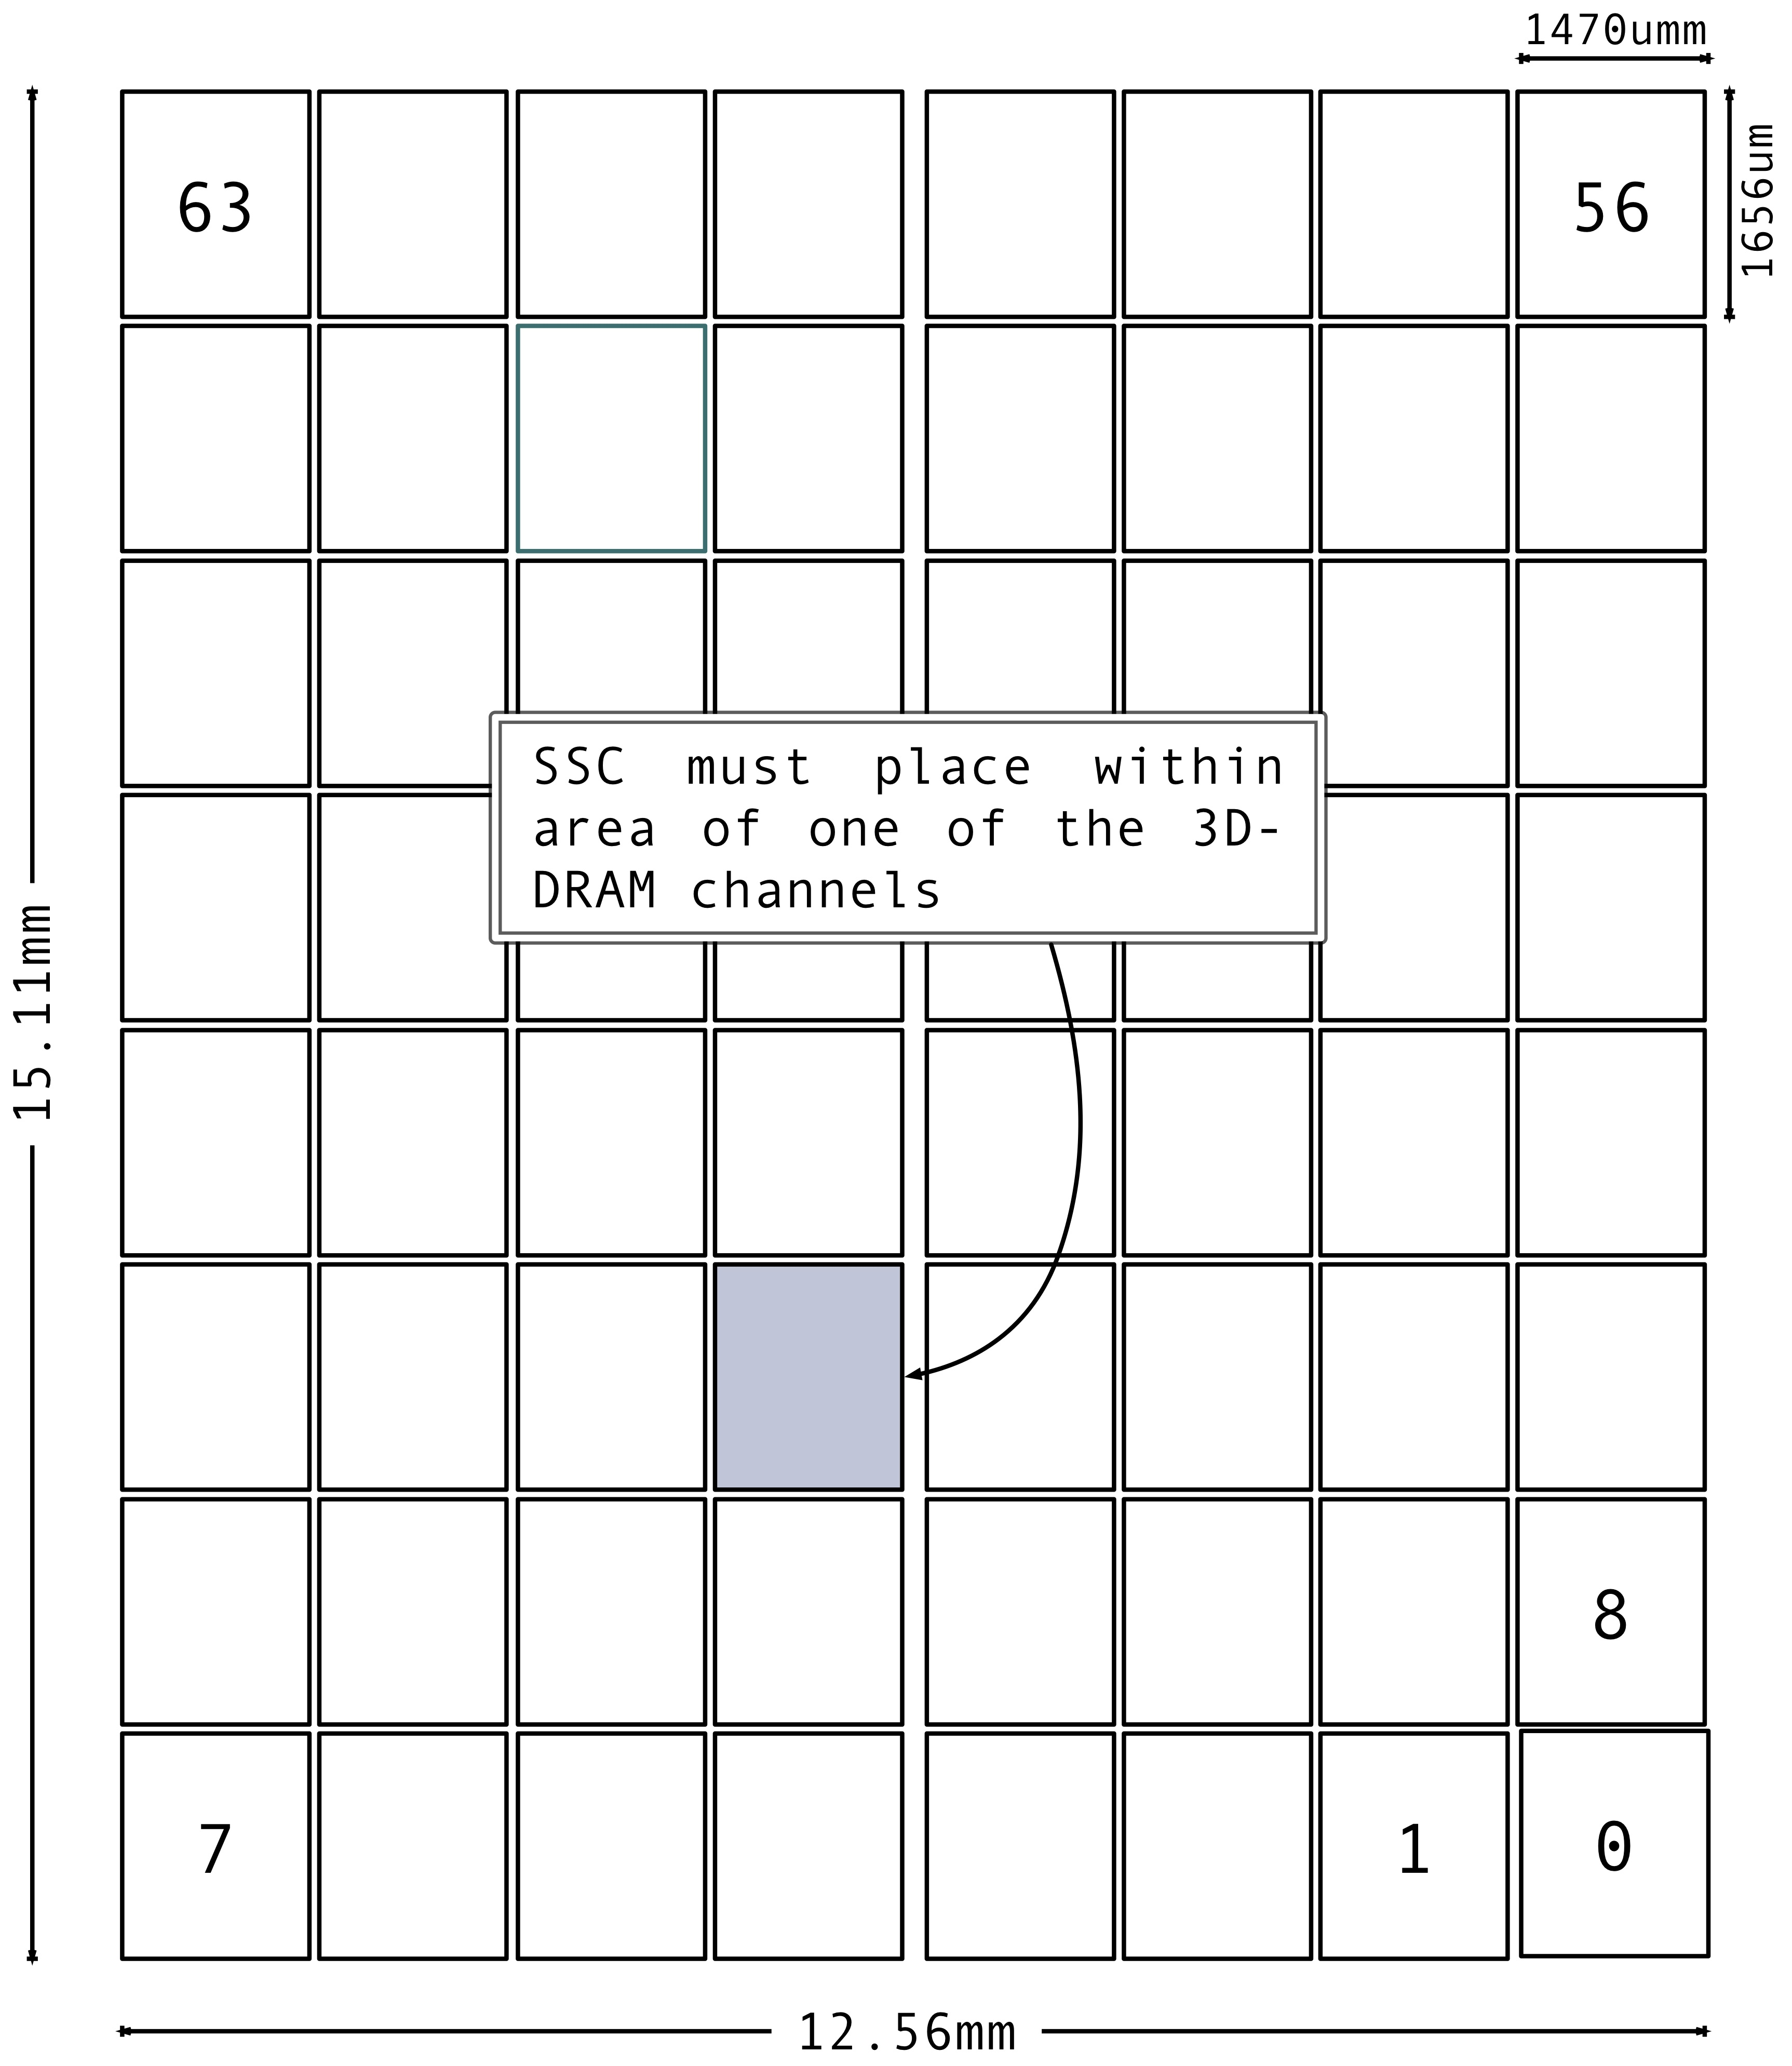
\includegraphics[width=.6\linewidth]{DiRAM4Layout.jpg}}
}
\caption{\ac{dram} Physical Interface Layout showing area for \ac{ssc}}
\label{fig:diram4Layout}
\end{figure}


% ----------------------------------------------------------------------------------------------------
\section{Manager Layer}
The Manager block is the main controller in the system. The operations required to process an \ac{ann} are formed from individual instructions which are decoded by the Manager. 
These instructions include descriptors to describe memory read operations, processing engine operations and memory write operations. The manager reads these system instructions from an instruction memory, decodes the instruction and configures the various blocks in the system.
The configuration includes:
\begin{itemize}
      \item initiate operand reads from \ac{dram}
      \item prepare the processing engine (\ac{pe}) to operate on the operands
      \item prepare the result processing engine to take the resulting neuron activations from the \ac{pe} and write those results back to the \ac{dram}
      \item replicate the resulting neuron activation's to neighbor managers for processing of other \ac{ann} layers
\end{itemize}

% ----------------------------------------------------------------------------------------------------
\section{Processing Layer}
\label{sec:Processing Layer}
The \ac{pe} is able to operate on data streamed directly from the \ac{dram} via the Manager layer. The \ac{pe} is configured by the manager to perform operations on the operand data streamed from the manager. In the baseline system, the main operation is to perform multiply-accumulates on 32 execution lanes of two operands. These operands typically are the pre-synaptic neuron activation's and the connection weights. The \ac{pe} also performs the activation function on the result of the MAC to generate the neuron activation value. These 32 activation values are sent back to the Manager layer.

% ----------------------------------------------------------------------------------------------------
\section{Layer Interconnect}
\label{sec:Layer Interconnect}

The layers are connected using through-silicon-vias (\ac{tsv}s) which provide high connection density, high bandwidth and low energy.
By ensuring the system stays within the 3D footprint ensures we can take advantage of the huge benefits provided by \ac{tsv}s.

% ----------------------------------------------------------------------------------------------------
\section{Inter-Manager Communication}
\label{sec:Inter-Manager Communication}

During configuration and/or computations, data must be transported between managers. This inter-manager communication is provided by an \ac{noc}.
When computing an \ac{ann} across multiple processing sub-systems, often neuron activation data must be shared between these \ac{ssc}s. The \ac{ssc} includes the \ac{dram} port, the manager and the \ac{pe}. An \ac{noc} within each management block communicates with each adjacent manager using a mesh network. This \ac{noc} has a forwarding table that can be reconfigured to provide more efficient routing for a given processing step.

A control and data flow diagram of the stack showing the 64 sub-system columns can be seen in figure \ref{fig:FlowDiagram}.
\begin{figure}[!t]
% the [] contains position info e.g. [!t] means here
\centering
\captionsetup{justification=centering}
\centerline{
\mbox{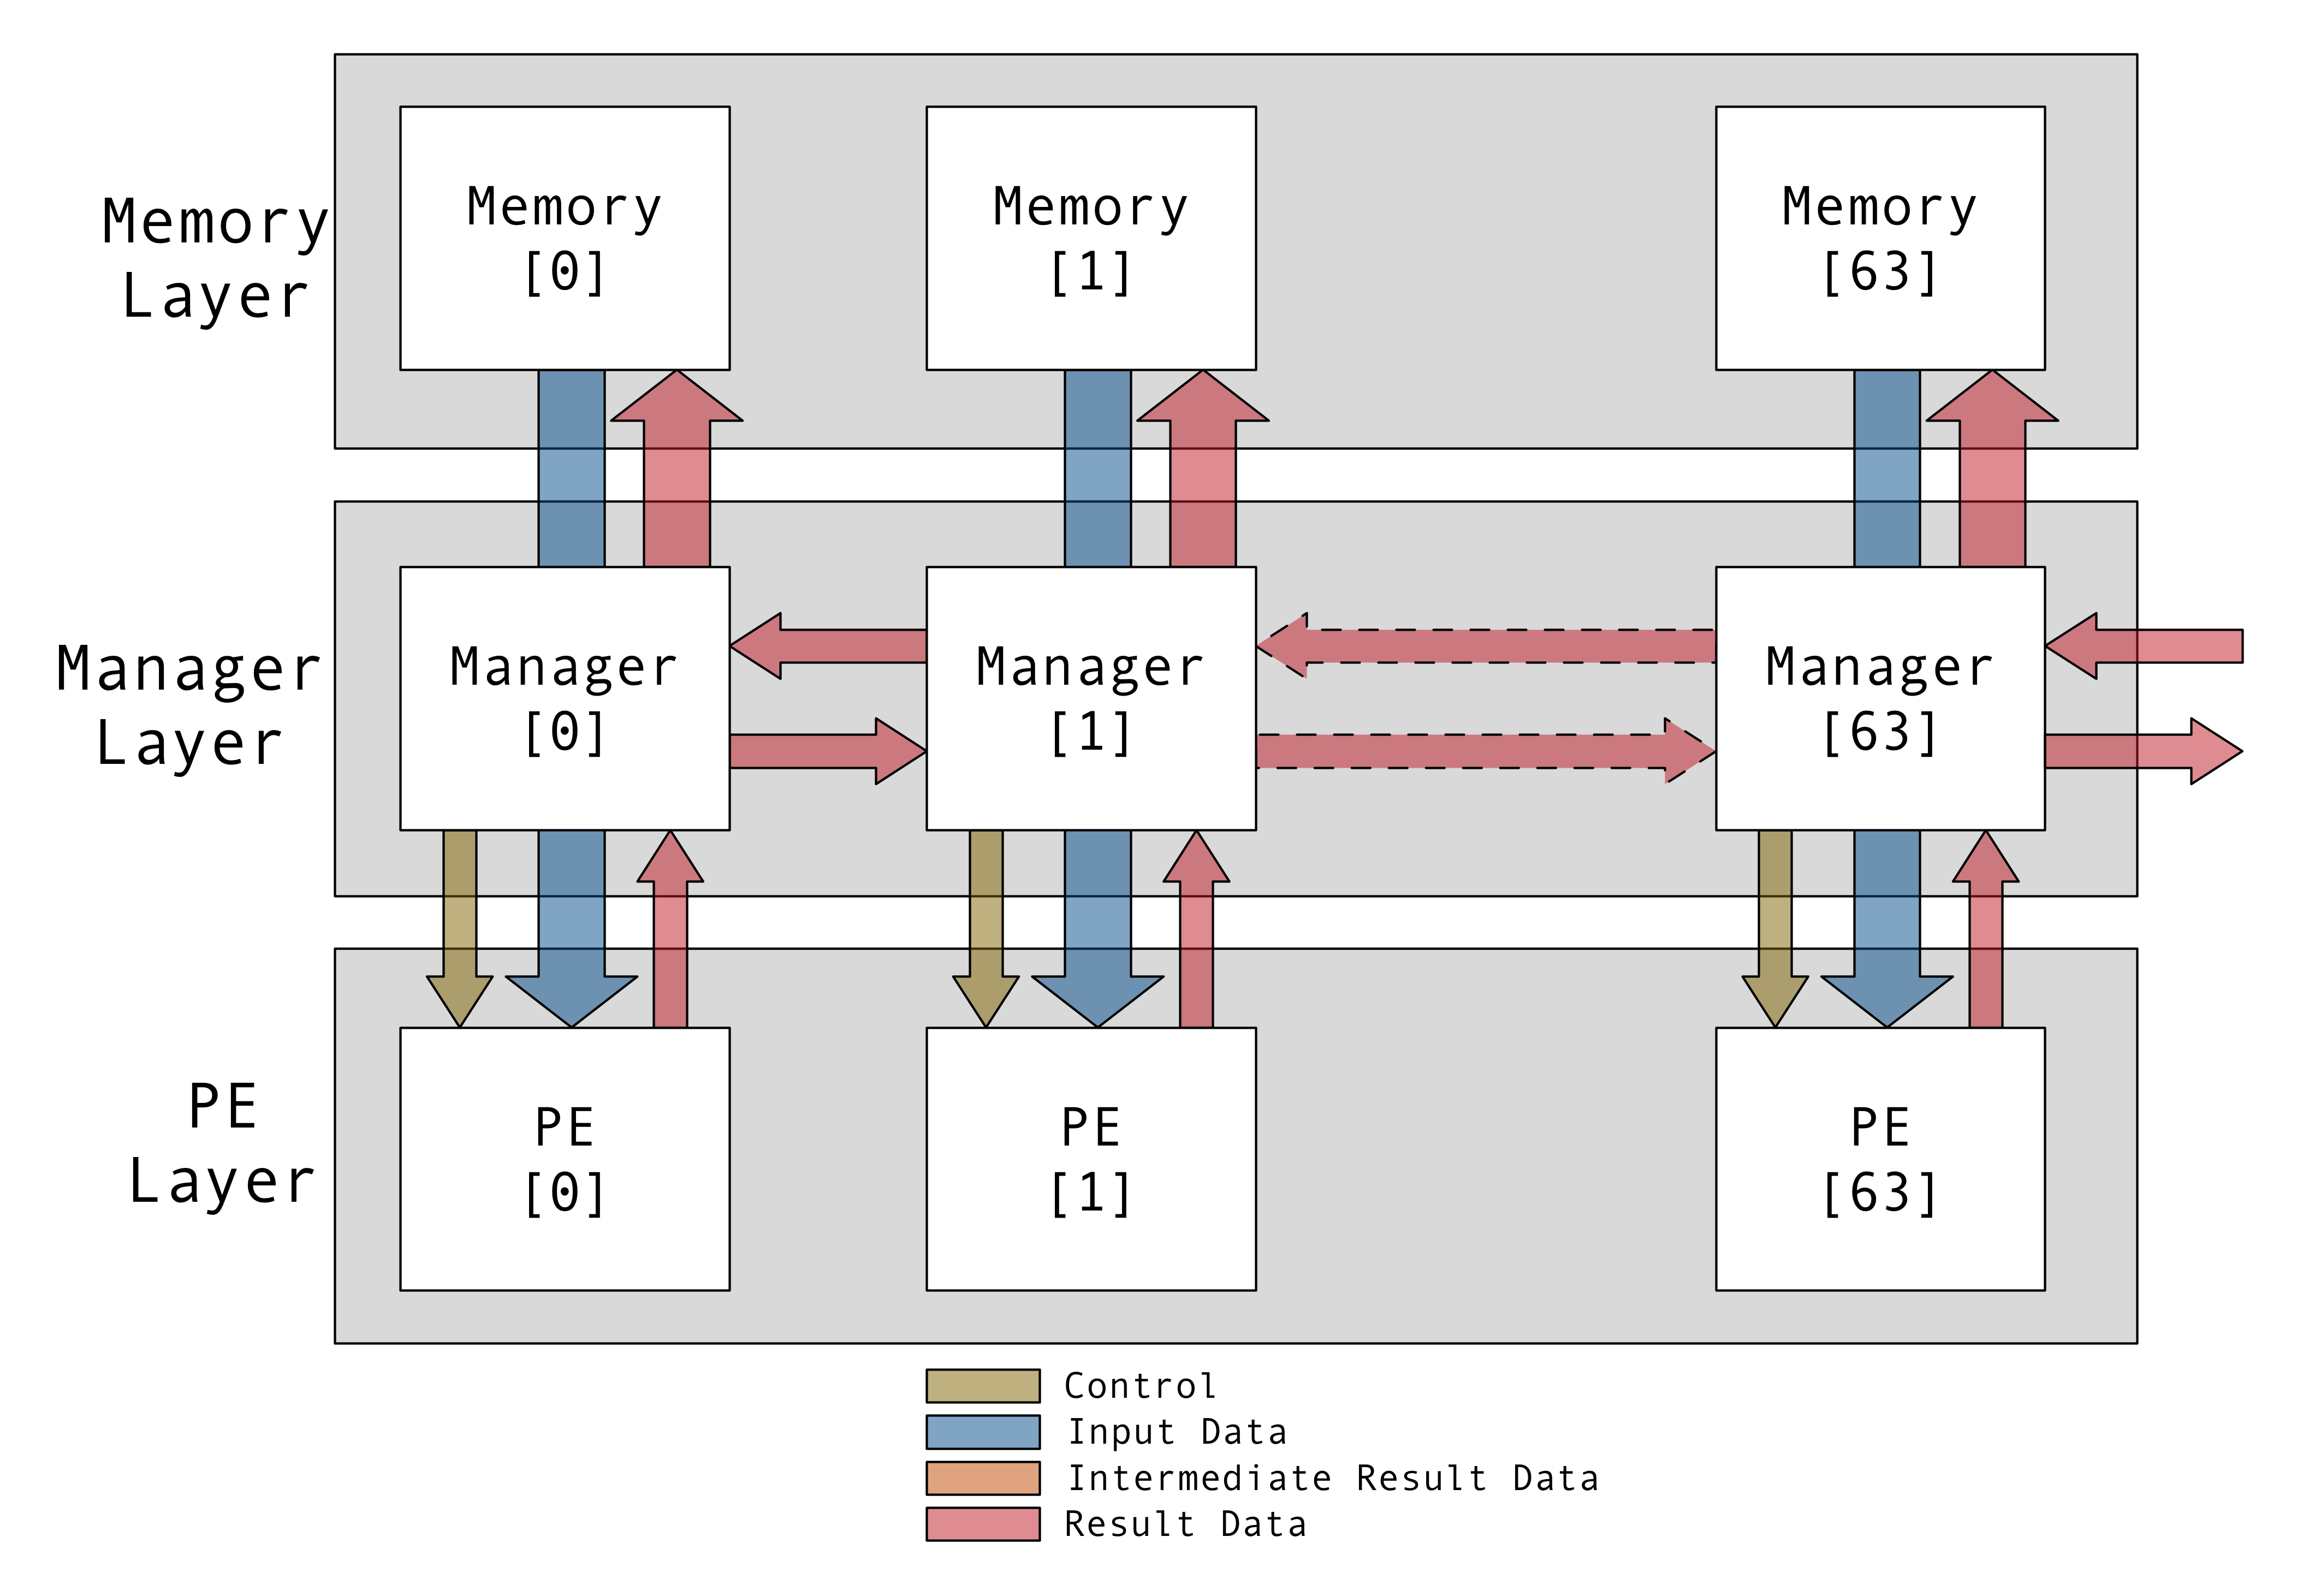
\includegraphics[width=.8\linewidth]{FlowDiagram.jpg}}
}
\caption{System Flow Diagram}
\label{fig:FlowDiagram}
\end{figure}



\section{System Operations}
\label{sec:System Operations}

In the context of this system and AN state calculation, the basic operations to determine the state of a neuron is to :
\begin{outline}
    \1 Inform the Manager and \ac{pe} which operations are to be performed
    \1 Tell the manager to access the states of the pre-synaptic neurons
    \1 Tell the manager to access the weights of the connections from the pre-synaptic ANs
    \1 Provide the pre-synaptic neuron weights and states to the processing engine execution lanes
    \1 Tell the manager where to store the resulting AN state back to memory
\end{outline}


This work has researched an instruction architecture to describe the above operations which are interpreted by the manager. 

In the baseline system, the manager is not responsible for performing specific algorithm operations but is responsible for coordinating the various data flows and configuration of the modules that make up the system.

The managers primary responsibility is:

\begin{outline}
    \1 Instruction decode
    \1 Internal Configuration messages
    \1 Operand read
    \1 Result write
\end{outline}

In the baseline system, the \ac{pe} is responsible for the main algorithm operations.

The \ac{pe} has three major blocks:

\begin{outline}
  %\setlength{\baselineskip}{10pt}
  %\setlength{\itemsep}{6pt}
    \1 Streaming operation function (\ac{stop})
      \2 Processes data from the manager on-the-fly without storing in local \ac{sram}
    \1 \ac{simd}
      \2 processes the data from the \ac{stop} function, usually neuron activation such as ReLu
    \1 DMA/local memory controller
      \2 transfer configuration data to \ac{pe} conroller or to store \ac{stop} results to a small local \ac{sram} which can be used for access by \ac{simd} or by the \ac{stop} function
\end{outline}
% ----------------------------------------------------------------------------------------------------
% ----------------------------------------------------------------------------------------------------
\subsection{Manager Operations}
\label{sec:Manager Operations}

% ----------------------------------------------------------------------------------------------------
\subsubsection{Instructions}
\label{sec:Instructions}
The instructions communicate:

\begin{outline}
  %\setlength{\baselineskip}{10pt}
  %\setlength{\itemsep}{6pt}
  %\setlength{\baselineskip}{10pt}
  %\setlength\itemsep{0pt}
  %\setlength{\partopsep}{0pt}
  %\setlength{\parskip}{0pt}
  %\setlength{\parsep}{0pt}
  %\setlength{\topsep}{0pt}
  %\setlength{\itemsep}{3pt}
  %\setlength{\itemindent}{\leftmargin}
  %\setlength{\leftmargin}{0pt}
        \1 To the Manager
            \2 ROI Storage descriptor
            \2 Parameter/Weight Storage Descriptor
                \3 Broadcast or Vectored
            \2 Result write storage descriptor
                \3 include descriptors for all destination managers
        \1 To the \ac{pe}
            \2 \ac{stop} operation
            \2 \ac{simd} operation
            \2 Number of active lanes
            \2 Operand Vector length
\end{outline}

Instructions include information to control the above operations.

Instructions contain sub-instruction called descriptors. These descriptors contain the information to control the various operations associated with the processing of a group of ANs.

The group size is related to the number of execution lanes which for the baseline system is 32. So a group can be anywhere from 1-32. It should be said that unless the group size consistently approaches 32 the system performance will be poor.

An instruction will typically have four descriptors:

\begin{outline}
\renewcommand{\outlinei}{enumerate}
    \1 Operation
    \1 Memory read for operand stream 0
    \1 Memory read for operand stream 1
    \1 Result write
\end{outline}

Note: An operand stream will be reffered to as an argument.

The instruction is actually an n-tuple where the tuple elements are descriptors and the number of elements can vary based on the operation being performed. In figure \ref{fig:instructionTuple} we see the format of a 4-tuple instruction which we use to perform an activation calculation for a group of neurons.

\begin{figure}[!t]
\centering
\captionsetup{justification=centering}
\captionsetup{width=.9\linewidth}
\centerline{
\mbox{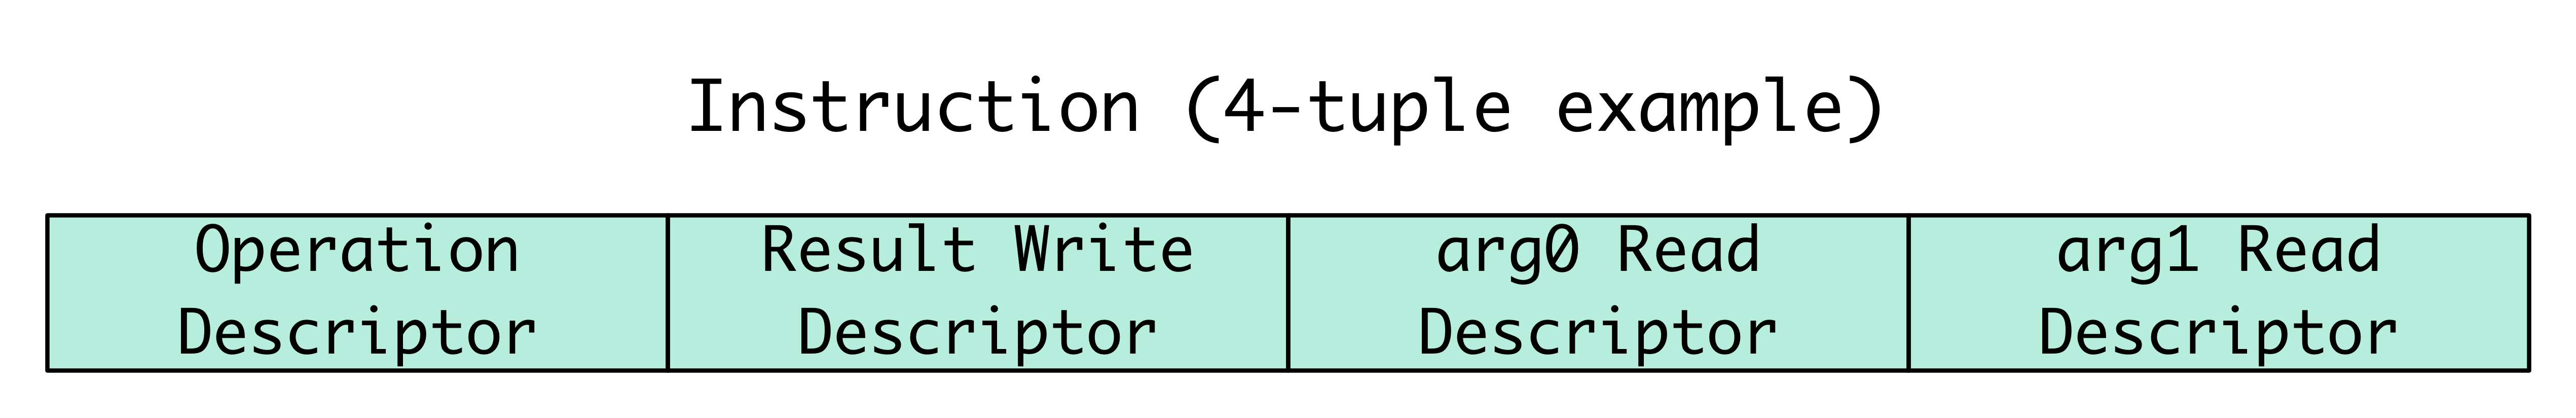
\includegraphics[width=.9\linewidth]{instructionTuple.jpg}}
}
\caption{Instruction 4-tuple}
\label{fig:instructionTuple}
\end{figure}

Now within a descriptor, we need to describe the various options such as storage descriptor pointer, number of operands etc..

Again, we employ a n-tuple format where the first tuple element describes the descriptors operation followed by an m-tuple whose elements contain the options required for the operation.

These option elements are a two-tuple with option and associated value.
In figure \ref{fig:descriptorTuple} we see the format of a 6-tuple descriptor.

\begin{figure}[!t]
\centering
\captionsetup{justification=centering}
\captionsetup{width=.9\linewidth}
\centerline{
\mbox{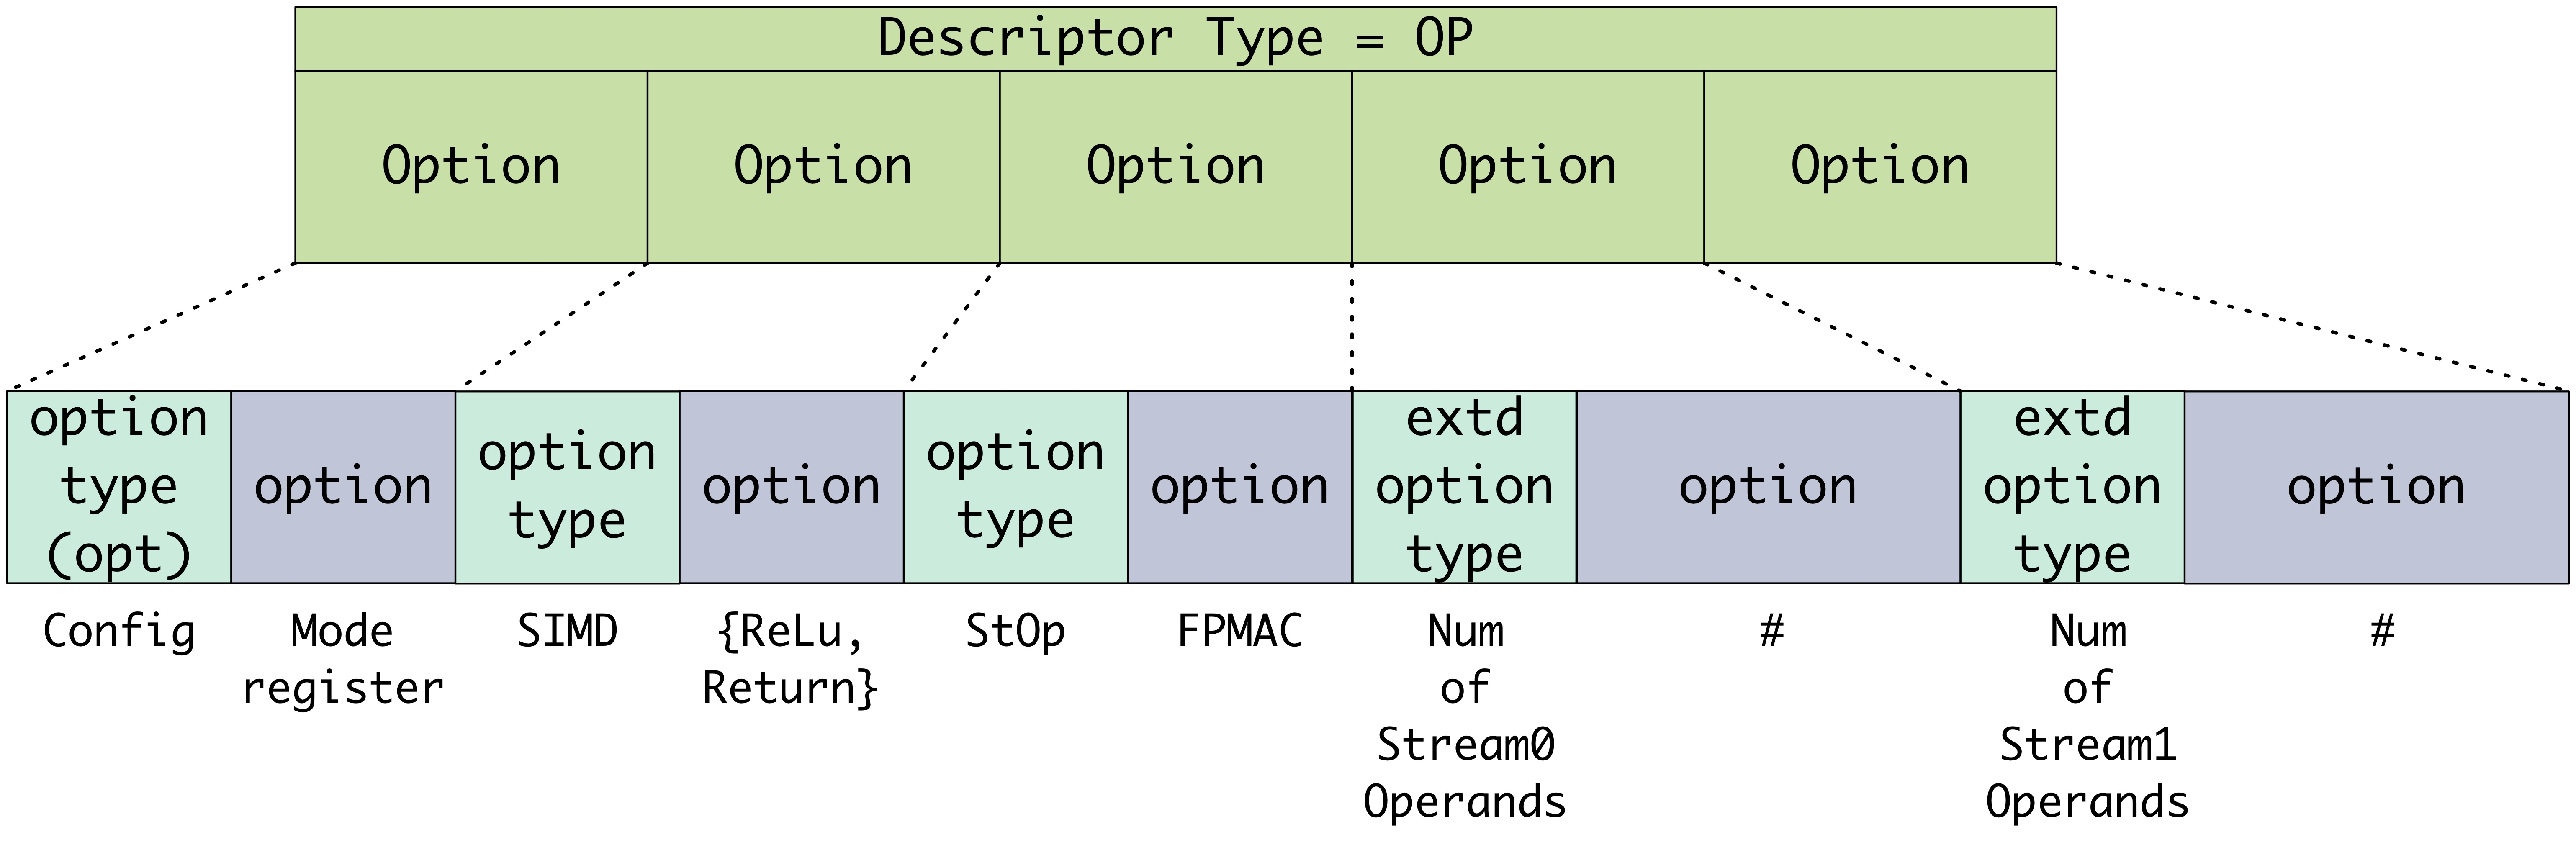
\includegraphics[width=.9\linewidth]{descriptorTuple.jpg}}
}
\caption{Descriptor 6-tuple}
\label{fig:descriptorTuple}
\end{figure}



% ----------------------------------------------------------------------------------------------------
\subsubsection{Accessing of Pre-synaptic AN states and connection weights}
\label{sec:AccessingANStates}

As was discussed previously, the ANN input and configuration is stored in main \ac{dram} memory. A part of the research is determining how to store the ANN input and parameters in such a way to effectively make use of main \ac{dram} bandwidth. To provide parameters for the up to 32 execution lanes within the \ac{pe}, we store the AN parameters in consecutive address locations. With one read to the \ac{dram}, we access 128 words. This provides four weights for each of the 32 ANs being processed. These weights are sent to each lane of the \ac{pe} over four cycles. We will discuss memory efficiency later, but by taking advantage of the multiple \ac{dram} banks along with pre-fetching and buffering, we are able to achieve relatively high efficiency of the available maximum bandwidth.

Although AN parameters (weights) are stored in contiguous memory locations, providing the input state to a particular AN presents us with an interesting problem.

Most often DNNs are represented by layers of ANs whose pre-synaptic neurons are from the previous layer. These previous layers represent the input to a given layer. The first layers input is the actual input to the ANN.


The input can be represented in the form of a 2-D array of AN states. For the sake of generality, the input array elements are considered as AN states.

Any given AN operates on a region of interest (ROI) within the input array.

In figure \ref{fig:roiStorage}, an input to a ANN layer in the form of a 2-D array along with the ROI of two ANs.

\begin{figure}[!t]
\centering
\captionsetup{justification=centering}
\captionsetup{width=.9\linewidth}
\centerline{
\mbox{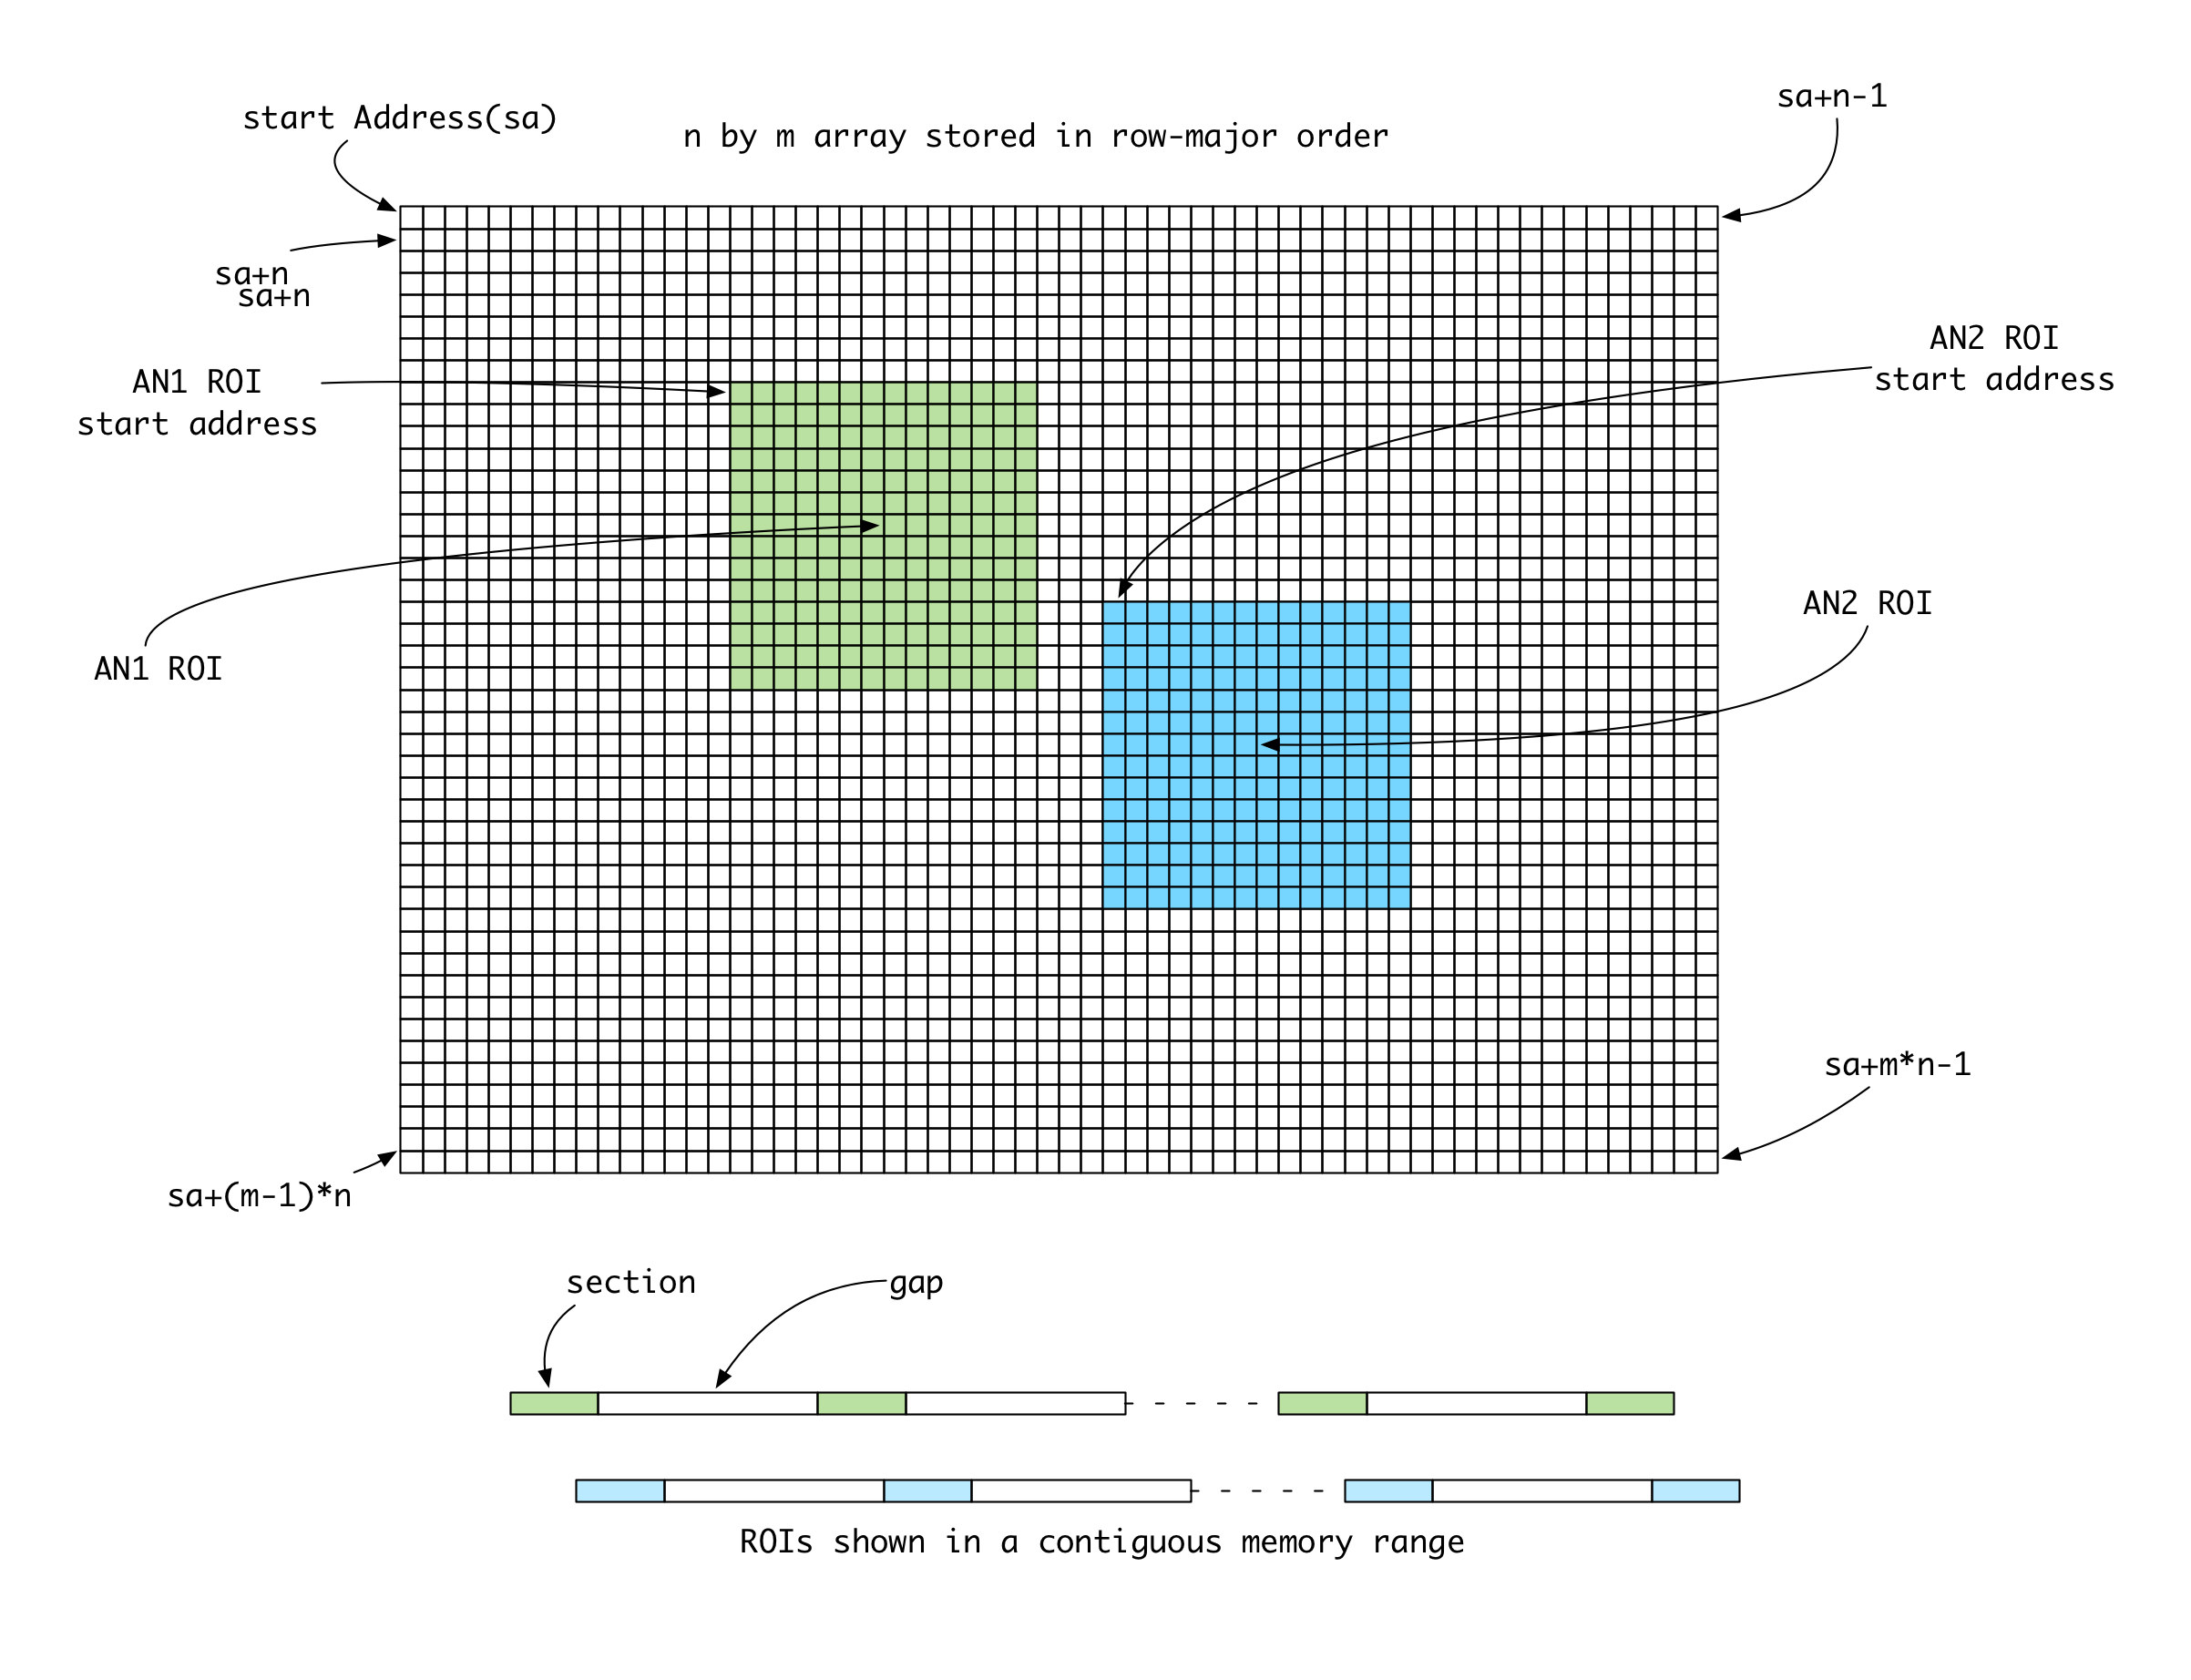
\includegraphics[width=.9\linewidth]{roiStorage.jpg}}
}
\caption{ROI Storage}
\label{fig:roiStorage}
\end{figure}

The various connection weights are stored in multiple contiguous sections. However, its not possible to arrange the input in such a way that each ANs ROI can be stored in contiguous memory locations. The figure above shows a typical ROI arrangement. Assuming the input array is stored in row-major order, an ROI is drawn from disjoint sections of memory. 
These disjoint sections contain a number of AN states and the sections are separated by a gap of a number of memory addresses. When the parameters are accessed when performing a particular operation, the memory controller within the manager must be informed of the start address and the lengths of the sections and gaps. Now this looks problematic, and it is, but in practice groups of ANs share a common ROI. So once we solve the problem of efficiently reading an ROI from the \ac{dram}, that ROI can be shared across a group of ANs

The read efficiency problem is solved by again taking advantage of the \ac{dram}s banks and pages.

This work proposes a data structure to describe these ROI storage locations.

Although disparate groups of ANs may have a different start addresses for their ROI, a commonality is observed in the ROI section lengths and gaps. So for each AN group, the groups ROI starting address is stored along with a pointer to a common set of section length/gaps. This structure is termed a storage descriptor.

This storage descriptor contains, amongst other things the start address of the ROI and a pointer to a section/gap descriptor. Many storage descriptors point to a common section/gap descriptor. This avoids having to have a unique section/gap descriptors for each AN group.

Figure \ref{fig:storageDescriptor} shows the structure of the storage descriptor. The SOD, MOD and EOD are used to delineate each descriptor in memory and stand for start-of-descriptor, middle-of-descriptor and end-of-descriptor.

\begin{figure}[!t]
\centering
\captionsetup{justification=centering}
\captionsetup{width=.9\linewidth}
\centerline{
\mbox{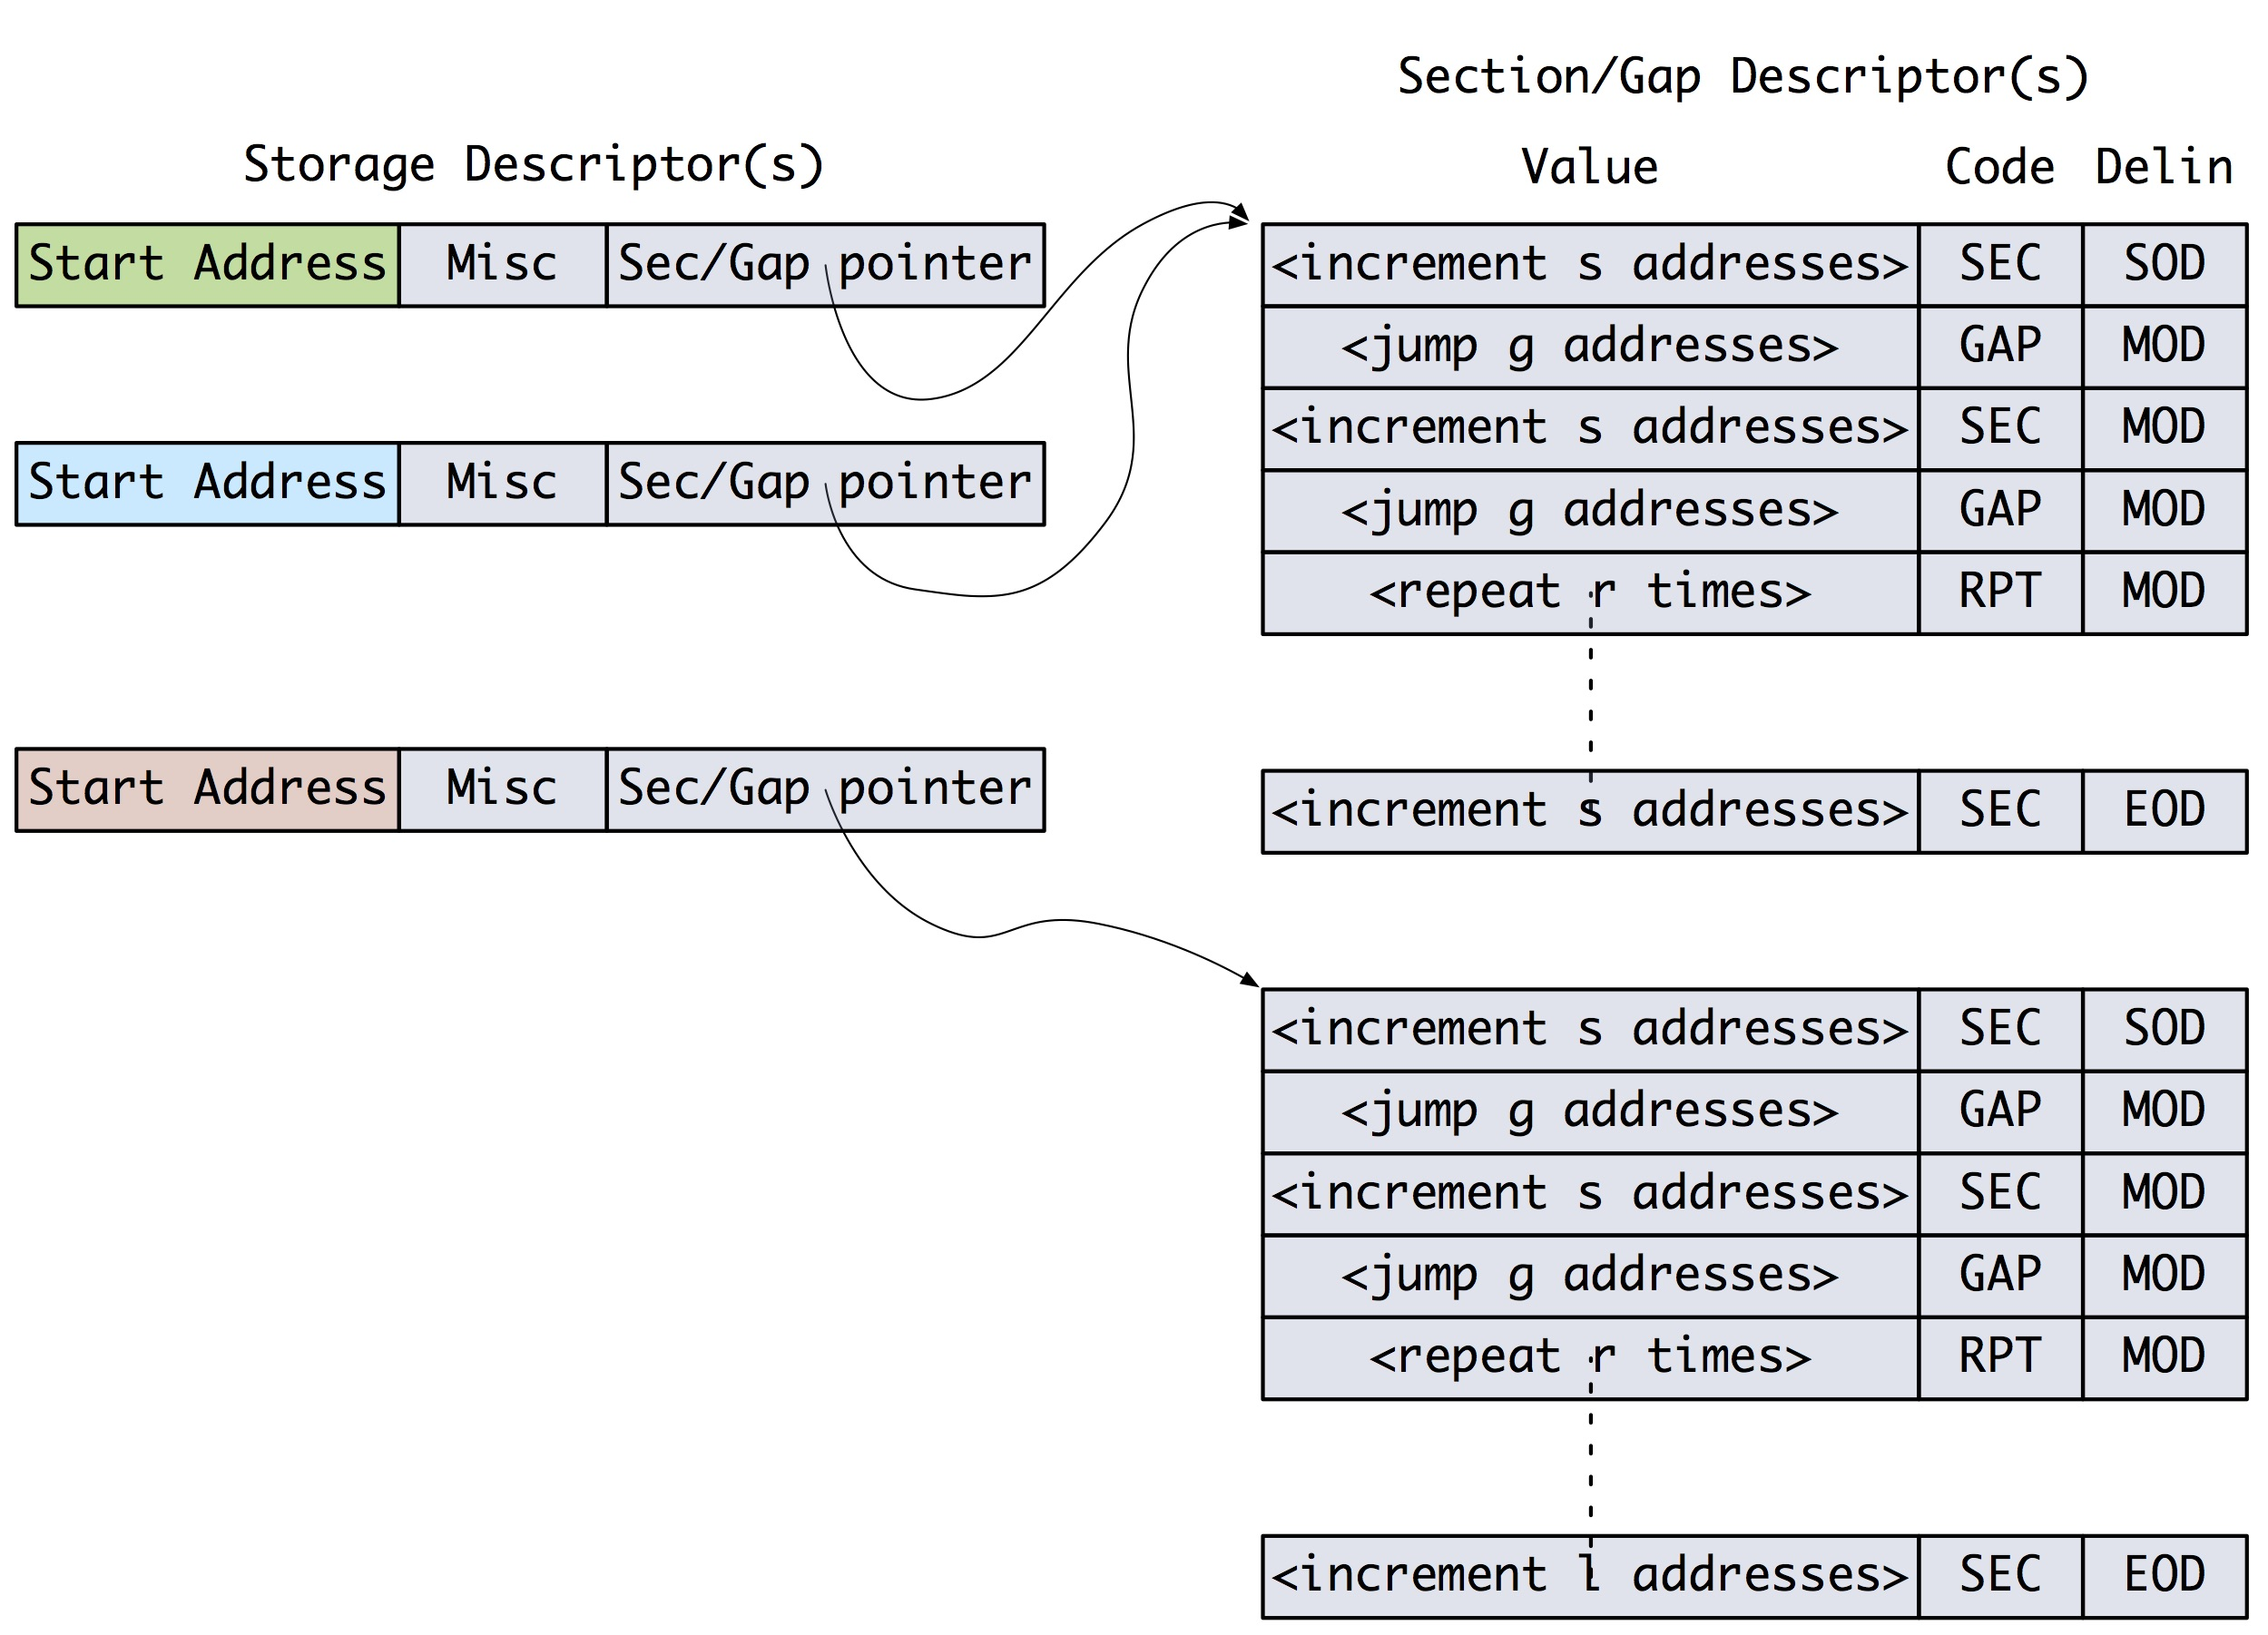
\includegraphics[width=.9\linewidth]{storageDesc.jpg}}
}
\caption{Storage Descriptor}
\label{fig:storageDescriptor}
\end{figure}

% ----------------------------------------------------------------------------------------------------
\subsubsection{Writing AN state results to memory}
\label{sec:writingANStates}

When the \ac{pe} has processed the group of ANs, the new AN states are sent back to the manager. The manager will store these back to \ac{dram} most likely in the array format as described earlier.

A significant difference taken advantage of is that for any given operation, the system is writing far less than is being read. For example, the ROI and parameters are usually vectors that will typically exceed 100 elements and in many cases much higher. When an operation is complete, in almost all cases one word per lane is writen back to main memory. 
Now that sounds like writing back has a very small impact on performance but with \ac{dram}s that's not always true.

When the system writes the result of an operation back to memory, it is often writing a small portion of a \ac{dram} page and the nature of the \ac{dram} protocol means this is a very inefficient use of \ac{dram} bandwidth. So although the amount of data written is small the performance impact cannot be ignored.

In addition, in many cases the results from a particular \ac{pe} has to be provided not only to the \ac{pe}s local manager but also to other managers. This is handled with a network-on-chip (NoC).

The result storage directives are communicated by using the same storage descriptor mechanism. However, the added complication is because the result will likely have to be replicated to other managers, the storage descriptors must be sent to all destination managers.


% ----------------------------------------------------------------------------------------------------
% ----------------------------------------------------------------------------------------------------
\subsection{PE Operations}
\label{sec:PE Operations}

% ----------------------------------------------------------------------------------------------------
\subsubsection{Streaming Operations (\ac{stop})}
\label{sec:streamingOps}
The operations performed by the \ac{stop} are primarily multiple-accumulate with a transfer to the \ac{simd} or to local memory.

Even though the baseline system focuses on the AN multiply-accumulate followed by a ReLu activation function, the system has built in flexibility into the \ac{stop} function to allow other functions to be added

In most cases, the \ac{stop} module will operate on the AN state and weights provided by the manager and provide the result to the \ac{simd}.
% ----------------------------------------------------------------------------------------------------
\subsubsection{SIMD}
\label{sec:SIMD}

The \ac{simd} is a 32-lane processor with some builtin special functions, such as the ReLu operation.

The \ac{simd} will take the result provided by the \ac{stop} and perform a ReLu. The result will, in most cases, then transmitted back to the manager.

% ----------------------------------------------------------------------------------------------------
\subsubsection{Configuration}
\label{sec:peConfiguration}

To configure these operations, two pointers are sent to the \ac{pe}. These pointers index into a small local memory which provides a program counter (\ac{pc}) to the function to be performed by the \ac{simd} and a configuration entry for the operation to be performed by the \ac{stop}.

The \ac{pe} is able to perform its operation concurrently on 32-lanes. However, there are cases when less than 32-lanes will be employed. This may occur if the number of ANs being processed is not modulo-32. In this case, the manager provides the number of lanes being processed for any given operation. In addition, the length of the vector of operands is also sent by the manager to the \ac{pe}.









%% Lee
%% In dissertation, change 
%    section* to chapter 
%    subsection* to section
%    subsubsection* to subsection


% #######################################################################################################################################
\section{Detailed System Description}
\label{sec:Detailed System Description}

A detailed flow diagram and block diagram of the sub-system column can be seen in figures \ref{fig:DetailedFlowDiagram} and \ref{fig:DetailedBlockDiagram} respectively.
\begin{figure}
% the [] contains position info e.g. [!t] means here
\centering
\captionsetup{justification=centering}
\captionsetup{width=.9\linewidth}
\centerline{
\mbox{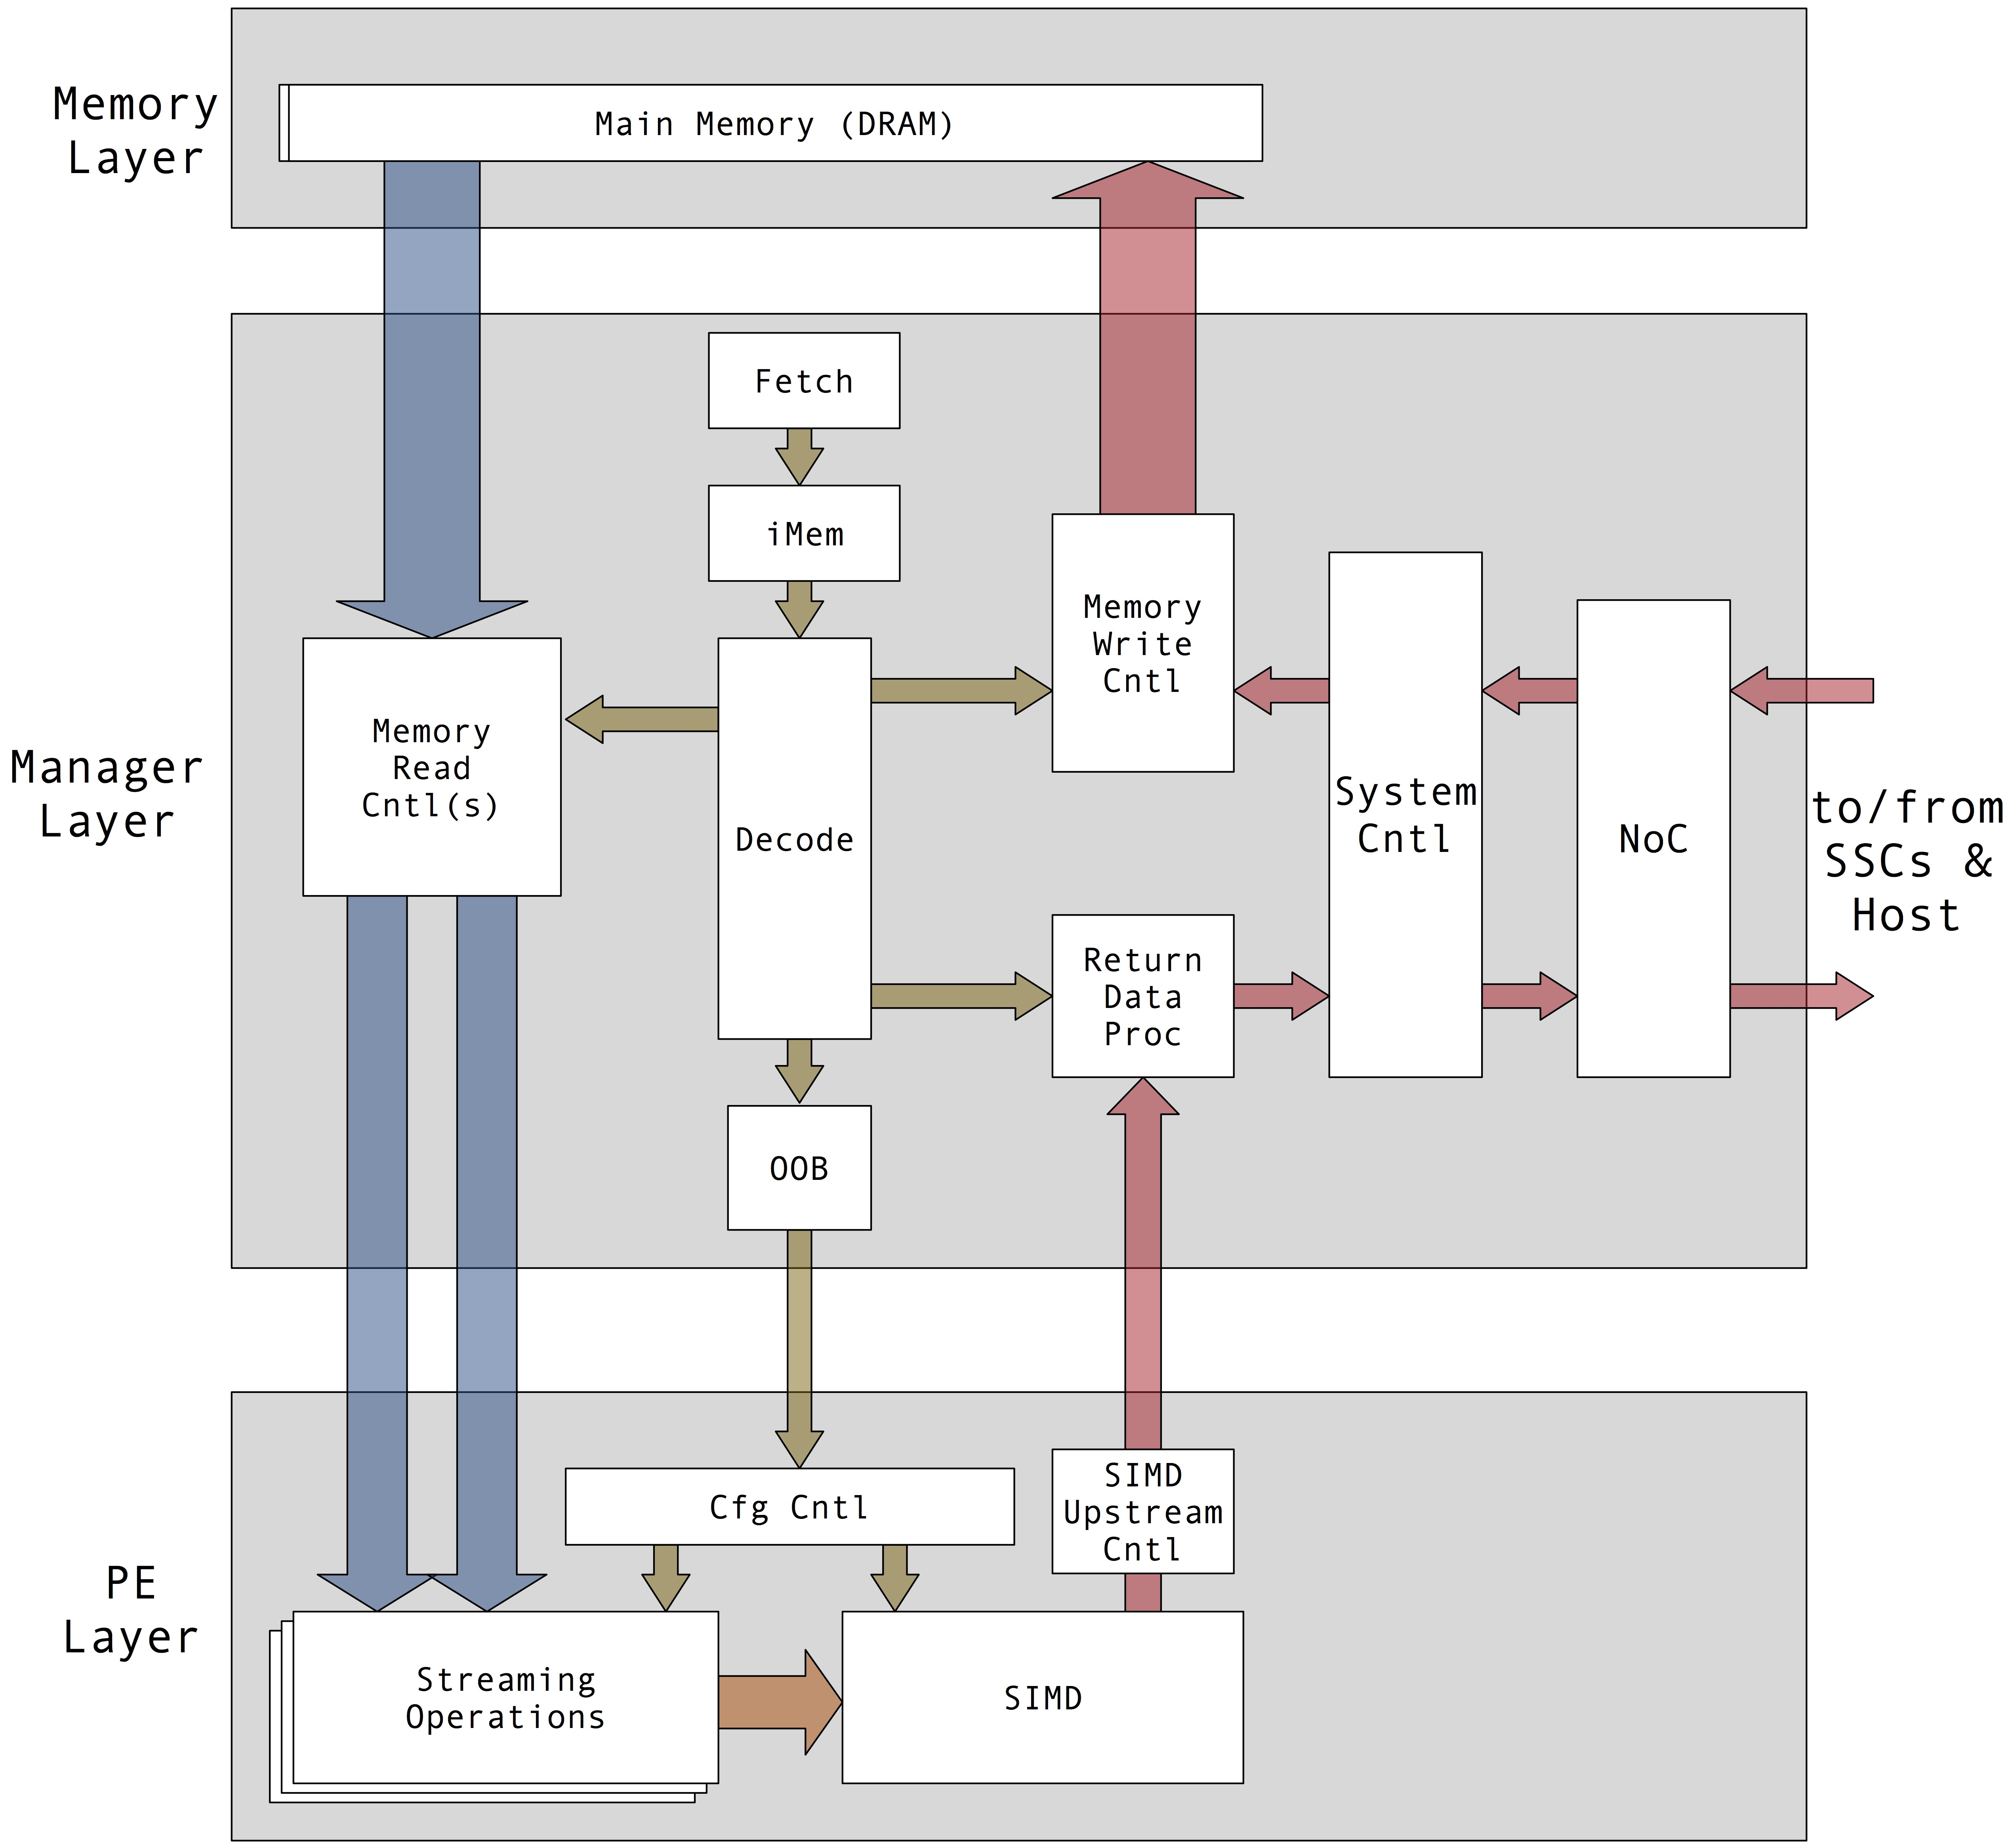
\includegraphics[scale=0.07]{DetailedFlowDiagram.jpg}}
}
\center\caption{Sub-System Column (SSC) Detailed Flow Diagram}
\label{fig:DetailedFlowDiagram}
\end{figure}

\begin{figure}[t]
% the [] contains position info e.g. [!H] means here
% H 	Place exactly at spot in source text
% h 	Place approximately at spot in source test
% t 	Place at top of page
% b 	Place at bottom of page
% p 	Place on page for floats only
% ! 	Override internal LaTeX parameters for determining float position
\centering
\captionsetup{justification=centering}
\captionsetup{width=.9\linewidth}
\centerline{
\mbox{
\includegraphics[angle=90, height=8in]{DetailedBlockDiagram.jpg}}
}
\center\caption{Sub-System Column (SSC) Detailed Block Diagram}
\label{fig:DetailedBlockDiagram}
\end{figure}

\subsection{Manager}
\label{sec:manager}

\subsubsection{Operation Decode}
\label{ssec:operationDecode}

In figure \ref{fig:DetailedBlockDiagram}, instructions are read from instruction memory and passed to the instruction decoder.

The operation tuple is decoded and a streaming operation (stOp) pointer and a SIMD operation pointer are sent to the PE inside an OOB control packet.

The stOp pointer specifies what streaming operation is to take place on the data directly streamed to the PE. In the baseline system, typically this would be a floating-point multiply accumulate on two arguments, the pre-synaptic neuron states and the pre-synaptic weights.

The SIMD pointer is essentially a program counter that will be invoked when the stOp result is passed to the SIMD.

Note that other types of stOp includes a NOP with a destination of local memory. This allows us to transfer block of instruction or data from the manager to the PE.


\subsubsection{Argument Decode}
\label{ssec:argumentDecode}
The instruction also includes argument descriptors. These descriptors include a storage descriptor pointers that point to a storage descriptor stored in local memory that encodes where data should be read from for the one or two arguments that will be streamed from DRAM to the stOp within the PE. In the case of a AN activation calculation, there are two arguments, the pre-synaptic neuron states and the pre-synaptic weights. The read storage descriptor pointers are passed to the Memory Read Controllers (MRC). The MRCs read the actual storage descriptor from their local memory and immediately start sending read commands to the memory via a Main Memory Controller (MMC). The MMC is not shown in the diagram but essentially takes the memory read requests and converts them into the DRAM read protocol.

As soon as read data is sent back to the MRC via the MMC, that data is aligned with the downstream bus and sent to the 32 Streaming Operations inside the PE.


\subsubsection{Result data Processing}
\label{ssec:resultDataprocessing}
The instruction also includes argument descriptors. These descriptors include a storage descriptor pointers that point to a storage descriptor stored in local memory that encodes where data should be read from for the one or two arguments that will be streamed from DRAM to the stOp within the PE. In the case of a AN activation calculation, there are two arguments, the pre-synaptic neuron states and the pre-synaptic weights. The read storage descriptor pointers are passed to the Memory Read Controllers (MRC). The MRCs read the actual storage descriptor from their local memory and immediately start sending read commands to the memory via a Main Memory Controller (MMC). The MMC is not shown in the diagram but essentially takes the memory read requests and converts them into the DRAM read protocol.

As soon as read data is sent back to the MRC via the MMC, that data is aligned with the downstream bus and sent to the 32 Streaming Operations inside the PE.


\subsubsection{Memory Write Controller}
\label{ssec:memoryWriteController}

The Memory Write Controller (MWC) receives data from to sources, the NoC via the MCNTL and the RDP.

In both cases, the MWC read the actual storage descriptor from their local memory and immediately start forming data that will be written back to main memory.

When the data is formed, a write command is sent to the memory via the MMC. Again, the MMC is not shown in the diagram but takes the memory write requests along with the data and converts them into the DRAM write protocol.

The MWC can only operate on one of the two sources at any one time. However, there are four 4096-bit holding registers where data is formed prior to the write request.

The holding registers have the potential in future to allow aggregation of data from one or more operations to allow a coalesced write back to main memory.


\subsection{Processing Engine}
\label{sec:pe}

\subsubsection{Configuration}
\label{ssec:peConfiguration}

A configuration controller within the PE (PE\_CNTL) takes the OOB packet from the Manager and extracts the stOp and SIMD operation pointers.

The stOp pointer is used to point to a local stOp configuration memory. The memory contains the various configuration data required by the streaming operation controller (stOp\_CNTL). The stOp\_CNTL is not shown.

The stOp\_CNTL configures the:

\begin{outline}
    \1 Operation type
    \1 Number of active execution lanes
    \1 Source of the argument data, which can be downstream data from the manager or from the small local SRAM
    \1 Destination of the result data, which can be the SIMD or the small local SRAM
\end{outline}

The SIMD operation pointer is sent to the SIMD.

\subsubsection{Streaming Operations}
\label{ssec:stOps}

The streaming Operations (stOp) are designed to operate on data passed from the Manager at or near line-rate. If line-rate cannot be maintained, a flow-control mechanism is employed to slow the data from the Manager.

Once the stOp has processed the data, it passes the result to the SIMD. Note in some cases the result can be placed in local SRAM or sent to both SIMD and SRAM.

It should also be stated that while the stOp is processing the current data, the SIMD may be operating on the result of the previous operation. It is expected the SIMD will have completed the previous operation before the stOp completes the current operation, but again, if necessary a flow control mechanism between SIMD and stOP will be engaged if the SIMD is not ready.

\subsubsection{SIMD}
\label{ssec:simd}

The SIMD takes the result data and performs the operation starting at the program counter (PC) indicated by the SIMD operation pointer provided by the PE\_CNTL.

The stOp provides the result to the SIMD via a local register. The result is also written, in most cases to the small local SRAM.

The SIMD performs the specified operation on the data provided by the stOp.

In most cases this will be the AN activation function and in the baseline system is the Rectified Linear function (ReLu).

When the SIMD has completed its operation, it passes the result to the SIMD Upstream controller to be returned to the Manager.

\subsubsection{Result Data}
\label{ssec:result}

The SIMD Upstream Controller (SUI) takes the data and encapsulates it in an Upstream packet. Included in the packet is the tag required by the Return Data processor within the Manager.



